\documentclass[10pt,landscape,a4paper]{article}
\usepackage[utf8]{inputenc}
\usepackage[ngerman]{babel}
\usepackage[T1]{fontenc}
%\usepackage[LY1,T1]{fontenc}
%\usepackage{frutigernext}
%\usepackage[lf,minionint]{MinionPro}
\usepackage{tikz}
\usetikzlibrary{shapes,positioning,arrows,fit,calc,graphs,graphs.standard}
\usepackage[nosf]{kpfonts}
\usepackage[t1]{sourcesanspro}
\usepackage{multicol}
\usepackage{wrapfig}
\usepackage[top=0mm,bottom=1mm,left=0mm,right=1mm]{geometry}
\usepackage[framemethod=tikz]{mdframed}
\usepackage{microtype}
\usepackage{pdfpages}

\usepackage{amsmath}
\usepackage{bm}

\let\bar\overline

\definecolor{myblue}{cmyk}{1,.72,0,.38}

\def\firstcircle{(0,0) circle (1.5cm)}
\def\secondcircle{(0:2cm) circle (1.5cm)}

\colorlet{circle edge}{myblue}
\colorlet{circle area}{myblue!5}

\tikzset{filled/.style={fill=circle area, draw=circle edge, thick},
    outline/.style={draw=circle edge, thick}}
    
\pgfdeclarelayer{background}
\pgfsetlayers{background,main}

\everymath\expandafter{\the\everymath \color{myblue}}
\everydisplay\expandafter{\the\everydisplay \color{myblue}}

\renewcommand{\baselinestretch}{.8}
\pagestyle{empty}

\global\mdfdefinestyle{header}{%
linecolor=gray,linewidth=1pt,%
leftmargin=0mm,rightmargin=0mm,skipbelow=0mm,skipabove=0mm,
}

\newcommand{\header}{
\begin{mdframed}[style=header]
\footnotesize
\sffamily
Cheatsheet
Joshua Hwang (44302650)
\end{mdframed}
}

\makeatletter % Author: https://tex.stackexchange.com/questions/218587/how-to-set-one-header-for-each-page-using-multicols
\renewcommand{\section}{\@startsection{section}{1}{0mm}%
                                {.2ex}%
                                {.2ex}%x
                                {\color{myblue}\sffamily\small\bfseries}}
\renewcommand{\subsection}{\@startsection{subsection}{1}{0mm}%
                                {.2ex}%
                                {.2ex}%x
                                {\sffamily\bfseries}}



\def\multi@column@out{%
   \ifnum\outputpenalty <-\@M
   \speci@ls \else
   \ifvoid\colbreak@box\else
     \mult@info\@ne{Re-adding forced
               break(s) for splitting}%
     \setbox\@cclv\vbox{%
        \unvbox\colbreak@box
        \penalty-\@Mv\unvbox\@cclv}%
   \fi
   \splittopskip\topskip
   \splitmaxdepth\maxdepth
   \dimen@\@colroom
   \divide\skip\footins\col@number
   \ifvoid\footins \else
      \leave@mult@footins
   \fi
   \let\ifshr@kingsaved\ifshr@king
   \ifvbox \@kludgeins
     \advance \dimen@ -\ht\@kludgeins
     \ifdim \wd\@kludgeins>\z@
        \shr@nkingtrue
     \fi
   \fi
   \process@cols\mult@gfirstbox{%
%%%%% START CHANGE
\ifnum\count@=\numexpr\mult@rightbox+2\relax
          \setbox\count@\vsplit\@cclv to \dimexpr \dimen@-1cm\relax
\setbox\count@\vbox to \dimen@{\vbox to 1cm{\header}\unvbox\count@\vss}%
\else
      \setbox\count@\vsplit\@cclv to \dimen@
\fi
%%%%% END CHANGE
            \set@keptmarks
            \setbox\count@
                 \vbox to\dimen@
                  {\unvbox\count@
                   \remove@discardable@items
                   \ifshr@nking\vfill\fi}%
           }%
   \setbox\mult@rightbox
       \vsplit\@cclv to\dimen@
   \set@keptmarks
   \setbox\mult@rightbox\vbox to\dimen@
          {\unvbox\mult@rightbox
           \remove@discardable@items
           \ifshr@nking\vfill\fi}%
   \let\ifshr@king\ifshr@kingsaved
   \ifvoid\@cclv \else
       \unvbox\@cclv
       \ifnum\outputpenalty=\@M
       \else
          \penalty\outputpenalty
       \fi
       \ifvoid\footins\else
         \PackageWarning{multicol}%
          {I moved some lines to
           the next page.\MessageBreak
           Footnotes on page
           \thepage\space might be wrong}%
       \fi
       \ifnum \c@tracingmulticols>\thr@@
                    \hrule\allowbreak \fi
   \fi
   \ifx\@empty\kept@firstmark
      \let\firstmark\kept@topmark
      \let\botmark\kept@topmark
   \else
      \let\firstmark\kept@firstmark
      \let\botmark\kept@botmark
   \fi
   \let\topmark\kept@topmark
   \mult@info\tw@
        {Use kept top mark:\MessageBreak
          \meaning\kept@topmark
         \MessageBreak
         Use kept first mark:\MessageBreak
          \meaning\kept@firstmark
        \MessageBreak
         Use kept bot mark:\MessageBreak
          \meaning\kept@botmark
        \MessageBreak
         Produce first mark:\MessageBreak
          \meaning\firstmark
        \MessageBreak
        Produce bot mark:\MessageBreak
          \meaning\botmark
         \@gobbletwo}%
   \setbox\@cclv\vbox{\unvbox\partial@page
                      \page@sofar}%
   \@makecol\@outputpage
     \global\let\kept@topmark\botmark
     \global\let\kept@firstmark\@empty
     \global\let\kept@botmark\@empty
     \mult@info\tw@
        {(Re)Init top mark:\MessageBreak
         \meaning\kept@topmark
         \@gobbletwo}%
   \global\@colroom\@colht
   \global \@mparbottom \z@
   \process@deferreds
   \@whilesw\if@fcolmade\fi{\@outputpage
      \global\@colroom\@colht
      \process@deferreds}%
   \mult@info\@ne
     {Colroom:\MessageBreak
      \the\@colht\space
              after float space removed
              = \the\@colroom \@gobble}%
    \set@mult@vsize \global
  \fi}

\makeatother
\setlength{\parindent}{0pt}


\begin{document}
%\footnotesize
%Template from tim-st/latex-cheatsheet
\small
\begin{multicols*}{4}
\section{Definitions and basic tools}
A \textbf{stochastic process} $(X(t), t \in T)$
is a collection of random variables indexed by
some indexed set T.
Think of an array (finite or infinite) that returns a ``random'' number
at each t.

A \textbf{state space} is defined as the set such that
all $X(t) \in E$.

\textbf{Characteristic Functions} are
defined as $\varphi_X(t) = \mathbb{E}\left[e^{itX}\right]$.
It is also $\varphi_X(-it) = M_X(t)$. Where $M_X(t)$ is the moment generating
function for $X$.

Recall the \textbf{Probability Generating Functions (PGF)}.
(It only works for discrete random variables) \\
$G_X(z) = \sum_{k=0}^\infty z^k \mathbb{P}(X=k)$
Also recall, $G'(0) = \mathbb{P}(X=1)$. And more generally,
$G^{(k)}(0) = k! \mathbb{P}(X=k)$.

Much like other transformations, if we find the PGFs are equal then they
are exactly equal.

We call a sequence of events \textbf{mutually exclusive} if the probability
of the intersection of events is equal to the product of probabilities,
$\mathbb{P}(\bigcap A_i) = \prod \mathbb{P}(A_i)$

Given a regular sequence of numbers that is fluctuating, we have an upper limit
given by the $\limsup$ and a $\liminf$ for the lower bound.

\textbf{Law of total probability} \\
$\mathbb{P}(A) = \sum_n \mathbb{P}(A|B_n) \mathbb{P}(B_n)$

\textbf{Law of total expectation} \\
$\mathbb{E}(A) = \mathbb{E}\mathbb{E}[A|B_n]$ \\
$\mathbb{E}(A) = \sum_i \mathbb{E}[A|B_n]\mathbb{P}(B_i)$

\textbf{Law of total variance} \\
$\text{Var}(S_n) = \mathbb{E}(\text{Var}(S_n | S_{n-1})) + \text{Var}(\mathbb{E}[S_n | S_{n-1}])$

\textbf{Markov's inequality}
For any random variable $X >= 0$ and any $a > 0$ \\
$\mathbb{P}(X \geq a) \leq \mathbb{E}(X)/a$

The proof of this is shown below, \\
$\mathbb{E}[X] = \mathbb{E}[X \, I\{X<a\} + X I\{X \, \geq a\}]$ \\
$\mathbb{E}[X] = \mathbb{E}[X \, I\{X<a\}] + \mathbb{E}[X I\{X \, \geq a\}]$ \\
$\mathbb{E}[X I\{X \, \geq a\}] > 0$ from initial conditions \\
$\mathbb{E}[X] \leq 0 + \mathbb{E}[X I\{X \, \geq a\}]$ \\
$\mathbb{E}[X] \leq 0 + a\mathbb{E}[I\{X \, \geq a\}]$ \\
$\mathbb{E}[X] \leq 0 + a\mathbb{P}(I\{X \, \geq a\})$

\textbf{Covariance} \\
$\text{Cov}(X,Y) = \mathbb{E}[XY] - \mathbb{E}[X]\mathbb{E}[Y]$

\textbf{Variance} \\
$\text{Var}(X) = \text{Cov}(X,X)$

\textbf{Spearman correlation coefficient} \\
$\rho = \frac{\text{Cov}(X, Y)}{\sqrt{\text{Var}(X) \text{Var}(Y)}}$

\textbf{Poisson pmf} is $\frac{\lambda^k e^{-k}}{k!}$. With mean and variance of $\lambda$.
Poisson PGF is $G(z) = e^{\lambda(z-1)}$.
\textbf{Binomial pmf} is ${}^nC_k p^k (1-p)^{n-k}$. Binomial PGF is $G(z) = ((1-p)+pz)^n$.
Uniform has variance $\frac{1}{12}(b-a)^2$.
\textbf{Exponential pdf} is $\lambda e^{-\lambda x}$. The mean is $1/\lambda$
the variance is $1/\lambda^2$.
\subsection{Matrices}
The sum of the eigenvalues is the same as the trace of the matrix.
The product of the eigenvalues is the same as the determinant.
If all the rows of the matrix sum to 1 then 1 is an eigenvalue.
\section{Branching Processes}
Each node in the branch has the probability of branches given by $X$ this is
called the offspring distribution.
We normally start at $S_0 = 0$, $S_k$ is the population at generation $k$. \\
$S_n = 1 + \sum_{k=1}^{S_{n-1}} X_k$

The expectation at every generation is given by, \\
$\mathbb{E}[S_n] = \mathbb{E}[X] \mathbb{E}[S_{n-1}]$

Considering we start at $S_0 = 1$ and $\mathbb{E}[X] = \mu$ we get, \\
$S_n = \mu^n$

Likewise for variance (with the same assumption that $S_0 = 1$) we get this
recursive formula where $\text{Var}(X) = \sigma$ \\
$\text{Var}(S_n) = \mu^{n-1} \sigma^2 + \mu^2 \text{Var}(S_{n-1})$

Evaluating this gets us, \\
$\text{Var}(S_n) =
\begin{cases}
\sigma^2 n & \text{if } n = 1 \\
\sigma^2 \mu^{n-1} \frac{1-\mu^n}{1-\mu} & \text{otherwise} \\
\end{cases}$

Probability of extinction is noted as $\eta_n$ which is the probability of
extinction at the $n$\textsuperscript{th} generation. We notate $\eta = \eta_\infty$.

From intuition we know that, \\
$\eta = 1$ when $\mu < 1$ \\
$\eta = 0$ when $\mu \geq 1$ \textbf{and} $\sigma = 0$.

In all other cases we find the following, \\
$\eta_n = G_X(\eta_{n-1})$

This means that the probability generating function for the offspring
distribution $X$ can be used to determined our $\eta$.

To find the probability of eventual extinction we take $\eta = G(\eta)$.
We should expect at least one solution of the form $G(1) = 1$. This is 
certain extinction resulting from the previous generations certain
extinction.

Interestingly, if a second equilibrium exists then that solution will be
stable and extinction is not stable.
\section{Discrete Time Markov Chain}
We define $(X_t, t\in T)$ where $X$ is the state at time $t$.
Markov processes must only be dependent on the immediate history.

$P_{ij}^m(n)$ means going from state $i$ at step $n$ to state $j$ at step $n+m$.
This notation doesn't matter since we just use these as matrix
multiplication. \\
$P^m(n) = P^1(n) \times P^1(n+1) \ldots P^1(n+m-1)$

Please note that $P^1(n) \neq P^1(m)$ since the transitions may change over
time.

Every column of the matrix determines ``where could I go given I'm in row $i$''.

$\pi$ is a row vector we position as $\pi P$ denoting the initial
distribution.

If we have countably infinite states then a matrix won't do and we'll need
to use linear operators and generate a function instead of just a matrix.

Just like the previous section we have
$\tau_y^{(k)} = \inf\{n > \tau_y^{(k-1)} : X_n = y\}$
Which refers to the amount of time, $n$, taken for us to reach state $y$.
$\tau_y^{(k)} > \tau_y^{(k-1)}$ for hopefully obvious reasons.

$r_{xy}^{(k)} = \mathbb{P}(\tau_y^{(k)} < \infty)$ refers the chance this
process goes on forever and touches $y$ at least $k$ times in finite time
knowing it started at state $x$. If $r=1$ then it's guaranteed we reach
state $y$. If $r=0$ then it's guaranteed to never reach $y$.

The \textbf{Strong Markov Property} states $r_{yy}^{(k)} = r_{yy}^k$. We
will attempt to demonstrate this for $r_{yy}^{(2)}$. \\
$r_{yy}^{(2)} = \mathbb{P}_y(\tau_y^{(2)} < \infty)$ \\
$= \mathbb{P}_y(\tau_y^{(2)} < \infty | \tau_y^{(1)} < \infty)
\times \mathbb{P}_y(\tau_y^{(1)} < \infty)$ \\
$= \mathbb{P}_y(\tau_y^{(2)} < \infty | \tau_y^{(1)} < \infty) \times r_{yy}$ \\
We know $\tau_y^{(2)}$ has the same distribution as $\tau_y^{(1)}$ 
that's why we're getting rid of the conditional but keeping the
distribution \\
$= \mathbb{P}_y(\tau_y^{(1)} < \infty | \tau_y^{(1)} < \infty) \times r_{yy}$ \\
$= \mathbb{P}_y(\tau_y^{(1)} < \infty) \times r_{yy}$ \\
$= r_{yy} \times r_{yy}$
$r_{yy}^{(2)} = r_{yy}^2$ 
\subsection{Infinite time}
Determining the infinite state of the Markov chain is difficult since we
have to $P^\infty$ to get it.
To do this quickly we must find the right eigenvectors $\vec{v}_\lambda$
generated from $P \vec{v}_\lambda = \lambda \vec{v}_\lambda$
and the left eigenvectors
$\vec{w}_\lambda$. We desire $\vec{w}_i \dot \vec{v}_i = 1$ but
$\vec{w}_j \cdot \vec{v}_i = 0$ when $i \neq j$.
Now we can write our matrix out as, \\
$P^n = \sum_{k=1} \lambda_k^n R_k$ where $R_k = \vec{v}_k \vec{w}_k$ \\
Since we're working with $P$ which has rows which sum to 1 we know one of
eigenvalues is always 1 thus, \\
$P^n = R_1 + \sum_{k=2} \lambda_k^n R_k$.

Another way to solve for infinite time is to take the fixed point solution,
$\pi P = \pi$.

Another is the use of \textbf{global balance equations}
$\sum_{x \in E} \pi_x P_{xy} = \pi_y$. This means that the state y is
equivalent to summing up every other state multiplied by the probability
our state $x$ goes to state $y$.

When global balance is too hard consider \textbf{local balance equations}.
$\pi_x P_{xy} = \pi_y P_{yx}$. A solution to the local balance will give a
solution to the global balance but not always the other way around. All local
balances are global balances but not all global balances are local balances.

\subsection{Categorising groups of states}
If $r_{yy} < 1$ then the chance of hitting state $y$ after every hit becomes
less and less likely. We call this $y$ a \textbf{transient state}.

If $r_{yy} = 1$ then we are always guaranteed to hit our states $y$. This is
called a \textbf{recurrent state}. When dealing with infinite states we
distinguish between \textbf{positive recurrent}, $\mathbb{E}_x[\tau_x < \infty]$
(expected time to return to $x$ starting from $x$), and \textbf{null
recurrent}, we don't expect to return in finite time.

More notation: if $r_{xy} > 0$ then we say that $x$ leads to $y$ and write $x \to y$.
If $x \to y$ and $y \to x$ we say that $x$ and $y$ communicate and write
$x \leftrightarrow y$.

This relation is transitive since $x \to y$ and $y \to z$ means $x \to z$.
\textbf{Proof}: If $x \to y$ then $r_{xy} > 0$ thus $\exists m \geq 1$ where
$\mathbb{P}_x(X_m = y) > 0$.
Likewise $y \to z$ gives $\exists n \geq 1$ and $\mathbb{P}_y(X_n = z) > 0$. \\
$\mathbb{P}_x(X_{n+m} = z) \geq \mathbb{P}_x(X_{n+m} = z | X_n = y) \mathbb{P}_x(X_n = y)$ \\
$= \mathbb{P}_y(X_{m} = z) \mathbb{P}_x(X_n = y) > 0$ \\
Thus $r_{xz} > 0$ and $x \to z$.

If $x$ is recurrent and $x \to y$ then $y$ is also recurrent \textbf{and} $y \to x$.

A communicating class is defined as a set of states that all communicate
with one another and don't communicate with external sets. Note that we
can have $x \to y$ leaving the communicating class.

If the entire state space is a communicating class then the state space is
called \textbf{irreducible}.

If $r_{xy} = 0$ $\forall y \in A^c$ where $A$ is the communicating class,
then we call $A$ \textbf{closed}. Additionally if $A$ is a single element
then $a \in A$ is called \textbf{absorbing}.

If $C$ is a finite, closed, communicating class then all states in this
family are recurrent.

The \textbf{period} of a recurrent state family is determined by gcd 
of the number of
hops required to return to a state (e.g. It takes 4,6,8 steps to return
to state $x$ means 2 is the period) (e.g. It takes 2,3,6 steps to return to
state $x$ means 1 is the period). If the period is 1 then we call it
\textbf{aperiodic}. Period is a class property since if $x$ has a period and
$x \leftrightarrow y$ then $y$ has the same period.

If our system is irreducible, positively recurrent and aperiodic then we
have a unique stationary distribution i.e. no matter what initial starting
position we always land back to the unique stationary distribution.
\subsection{Big brain confusing (Reversible)}
We can construct a new path through a Markov chain that takes an original
path $x_i$ and reverses it, $y_m = x_{n-m}$.
A \textbf{reversible} chain is when we cannot determine which way is the
reverse. This only occurs when the distribution is stationary.

\textbf{Kolmogorov cycle condition} states that $X$ is irreducible and
reversible \emph{iff} $P_{ij} > 0$ implies that $P_{ij} > 0$ and for any
loop of states (which we can get to) it holds that
$\prod_{i=1}^n p_{x_i x_{i-1}} = \prod_{i=1}^n p_{x_{i-1} x_i}$.

If Kolmogorov cycle condition holds then $X$ has a stationary distribution.

If $X$ is irreducible and positive recurrent then there is a unique
stationary distribution. Moreover if $X$ is aperiodic then all distributions
lead to the unique stationary distribution.

\section{Homogeneous Poisson Processes}
We denote $N(t)$ to be the current count at continuous time $t$.
We note $T_i$ the time of the $i$\textsuperscript{th} jump.
$A_i$ represents the interval between jumps ($A_2 = T_2 - T_1$).

An obvious insight is $\{N(t) \geq n\} = \{T_n \leq t\}$.

We note that $N(I) \sim Poi(\lambda \times |I|)$ where $I$ is some interval.
Also note that all disjoint intervals will be independent.
We denote a specific interval by $N(s,t+s] := N(t+s) - N(s)$.

$A_i \sim exp(\lambda)$.

From simple observation of $\mathbb{P}(N(t+h) = m | N(t) = n)$ we can classify
four possibilities, \\
If $m < n$ then there's no chance \\
If $m = n$ then $1 - \lambda h + o(h)$ \\
If $m = n+1$ then $\lambda h + o(h)$ \\
If $m > n+1$ then $o(h)$

$\bm{o(h)}$ is just a function that ensures that if $h \to 0$ then $o(h)/h \to 0$.

The times of our $T_i$s has the same distribution as an \emph{ordered} list of
uniform random variables.
\subsection{Ordered Uniform Random Variables}
The PDF of $n$ random variables is $1/t^n$ where $t$ is the domain of the
random variable.

In comparison, sorted random uniforms have $n!/t^n$ in the
region that makes sense and 0 everywhere else. To understand why consider a load
of uniform random variables have been realised. There are $n!$ ways to order
them and we funnel all $n!$ possibilities into the same sorted list thus
$n! \times 1/t^n$.

Adding two Poisson processes with parameters $\lambda_1$ and $\lambda_2$ will
give another Poisson process with $\lambda_1 + \lambda_2$. This property is
known as the \textbf{superposition of Poisson processes}.
\section{Non-homogeneous Poisson Processes}
If our $\lambda$ is variable through time then,
$N(a,b] \sim Poi\left(\int_a^b \lambda(s)\,ds\right)$

$A_i$s are no longer exponentially distributed, no longer memoryless and
not independent. Disjoint intervals are \emph{still} independent
i.e. $N(a,b]$ and $N(b,c]$ are independent. Superposition still holds as well.
\section{Continuous Time Markov Chains}
We redefine the transition probability as $p_t(i,j) = p(X_t = j | X_0 = i)$

All challenges in this course assume the \textbf{standard property} holds,
as time interval $\to 0$ our probability $\to 0$ for all states but itself.

The idea of periodic/aperiodic loses meaning in continuous time. We also
redefine $r_{x,x}$ as only the chance of return and not the chance of staying
since we now have a waiting time.

If the CTMC is irreducible and recurrent then no matter what starting position,
$\lim_{t\to\infty} \mathbb{P}_x(X_t = y) = \pi_y$.

We can actually split the time interval into disjoint parts which means we
can do same to our transition matrices,
$P_{t+s} = P_s P_t$

We define a function $h(w) = \mathbb{P}(W_0 > w | X_0 = i)$ which is the
probability that our \textbf{wait time} $W_0$ is greater than $w$.
Just like with the matrices, $h(u+v) = h(u) h(v)$.
From this the only solution is $h(u) = e^{-cu}$ for some constant $c$.

For homogeneous time $h(u)$ follows an exponential distribution. We define
$q_x$ as the exponential's parameter at state $x$.

$K_{x,y}$ is the probability we jump from $x$ to $y$ and can be used to
construct the \textbf{jump chain matrix}.
We then define $q_{x,y} = q_x K_{x,y}$.
Redefining, $K_{x,y} = \frac{q_{x,y}}{q_x} + I\{x=y\}$.
Note that $\sum_y K_{x,y} = 1$.

If we have reached the infinite jump in finite time,
$\mathbb{P}(\lim_{n\to\infty} T_n = \infty) = 0$, then we call this an explosion.

On the other hand, $\mathbb{P}(\lim_{n\to\infty} T_n = \infty) = 0$, is
considered regular.

Much like the p-matrix for transitions in discrete time Markov chains we define
q-matrix as filled with the $q_{x,y}$ parameters with $q_{x,x} = -q_{x}$.

Due to our choice of $q_{x,x}$ the matrix is singular and has an eigenvalue of 0.

\subsection{Galaxy brain confusing (Kolmorgorov Backward Equations)}
We can differentiate the matrix with respect to time to get,
${P'}_t = Q P_t$. This is known as the Kolmorgorov Backward Equations.

Under the finite and ``standard'' properties the matrices are actually commutative,
${P'}_t = P_t Q$. Additionally, $P_t = e^{tQ}$ is the unique solution in the
finite case. This is solved via the Taylor expansion,
$e^{tQ} = \sum_{k=0}^\infty \frac{(tQ)^k}{k!}$.

\subsection{Infinite time}
We could spectral decomposition our $P_t$ matrix giving us,
$R_1 + \sum_{k=2}^p e^{\alpha_k t} (\cos(\beta_k t) + i \sin(\beta_k t))$.
Which is the softened spring equation.

Alternatively, we use q-matrix. Solving, $\pi Q = 0$, gives us the solution to
$\pi P_t = \pi$. Note this only works if $P_t = e^{tQ}$ and doesn't work the
other way around.

If we could decompose the q-matrix into $D(K-I)$ where $K$ is the
\textbf{jump chain matrix}. $I$ is the identity and $D$ is the diagonal
with the exponential holding times. By taking the rows of $K$ denoted as
$\nu$ we can get the limiting distribution, \\
$\pi_x = \frac{\nu_x/q_x}{\sum_y \nu_y/q_y}$

If the denominator ever goes to $\infty$ then the correct solution is a 0 vector.
\section{Queueing theory}
Queueing systems are a type of \textbf{life-death process}.
Think of them like extensions
of counting processes where we have a single chain that only goes up with $\lambda_i$
and down one with $\mu_i$.

We denote a queue system via M/M/c as a Poisson Process queue with c servers.

With $c=1$ we have a common $\lambda$ and a common $\mu$. Our limiting distribution
becomes,
$\rho = \lambda/\mu$ and $\pi_i = \frac{\rho^i}{\sum_k^\infty \rho^k}$.
Since we have a geometric sum on the bottom this can only occur is $\rho < 1$ or
$\lambda < \mu$. In total we get $\pi_i = \rho^i(1 - \rho)$.

Under $c=\infty$, as more customers arrive the $\mu$s increase.
1 customer $\mu_1 = \mu$. 2 customers $\mu_2 = 2\mu$.
3 customers $\mu_2 = 3\mu$. 4 customers $\mu_2 = 4\mu$ etc. Our limiting distribution
becomes $\pi_i = \frac{\rho^i e^{-\rho}}{i!}$.

In general we're solving for
$\pi_i = \frac{\prod_{k=1}^n \frac{\lambda_{k-1}}{\mu_k}}{1+\sum_{n=1}^\infty \prod_{k=1}^n \frac{\lambda_{k-1}}{\mu_k}}$.
Ensuring the denominator doesn't explode to infinity.

\subsection{Kolmogorov Cycle Condition}
Consider a cycle chain where all states are connected to the two neighbours
and the ends of our chain are connected. The probabilities don't need to be the
same only non-zero.

Kolmogorov Cycle Condition states that if, 
$\prod_{i=1}^n q(x_{i-1}, x_i) = \prod_{i=1}^n q(x_{i}, x_{i-1})$, then there
exists solutions to local (aka \textbf{detailed) balance equations}. But now you
can use the $q$s to do it, $\pi_x q_{xy} = \pi_y q_{yx}$.
\section{Probability Measure Theory}
A probability space is made from three things,
$\Omega$ the set of all possibilities,
$\mathcal{F}$ the \textbf{event set},
$\mathbb{P}$ a \textbf{measure}.
\subsection{Event sets}
An event set must have the following;
must contain the empty set, the complement must exist for each element,
closed under unions. An event set is also called an \textbf{algebra}.
The most natural choice of $\mathcal{F}$ is the power set of $\Omega$.

We call a set of subsets a \textbf{monotone class} if there is some ordering
to the subsets (e.g. each is a subset of the consecutive).

We define \textbf{$\bm{\sigma}$-algebra} if $\Omega$ is in the event set and
the infinite union of elements is closed. In fact, it's a $\sigma$-algebra
\emph{iff} it's an algebra and a monotone class.
A $\sigma$-algebra is an algebra but not always the other way around.

The intercept of $\sigma$-algebras is also a $\sigma$-algebra. This is not
always true for the union however.

The \textbf{Borel $\bm{\sigma}$-algebra ($\bm{\mathscr{B}}$)} 
is a special type of $\sigma$-algebra
that attempts to work for the uncountably infinite, i.e. the real numbers. Within
$\mathscr{B}$ contains all possible intervals (both closed and open).
\subsection{Kolmogorov axioms of probability}
The axioms are:
$\mathbb{P}(\Omega) = 1$, \\
$\mathbb{P}(A) \geq 0 \quad \forall A \in \mathscr{F}$, \\
if $A_i$ are mutually disjoint events then
$\mathbb{P}(\bigcup^\infty A_n) = \sum^\infty \mathbb{P}(A_n)$

\textbf{Boole's inequality}
$\mathbb{P}(\bigcup^\infty A_n) \leq \sum^\infty \mathbb{P}(A_n)$ where $A_i$ might
not be disjoint.

\textbf{Continuity from below}
If $A_1 \subseteq A_2 \subseteq A_3 \ldots$
then $\mathbb{P}(A_n) = \mathbb{P}(\bigcup^\infty A_i)$.

\textbf{Continuity from above}
If $A_1 \supseteq A_2 \supseteq A_3 \ldots$
then $\mathbb{P}(A_n) = \mathbb{P}(\bigcap^\infty A_i)$.

Consider a sequence of events much like $A_1, A_2 \ldots$.
An element can exist in all sets in the sequence (\textbf{infinitely often})
this is the set analogue of $\limsup$,
or they exist in a few but still countably infinite number of sets
(\textbf{all but finitely many}) defined as the $\liminf$.

In notation, \\
$\{A_n\ i.o.\} = \bigcap_{n\geq 1}\left(\bigcup_{n \geq m}\ A_n\right)$
which means we're taking the union of the tail sequence then checking if we were
to intersect all of them we would find elements which appear infinitely often.

$\{A_n\ a.b.f.m\} = \bigcup_{m\geq 1}\left(\bigcap_{n\geq m}\ A_n\right)$
Consider all possible tails $A_n$. We take all the tails that contain surviving
elements and collect them.

Not only but these definitions means,
$\liminf A_n = (\limsup A_n^c)^c$. Also, $\{A_n \ a.b.f.m.\} \subseteq \{A_n \ i.o.\}$.

\textbf{Borel-Cantelli Lemma}
If $\sum\mathbb{P}(A_n)$ is non-infinite then $\mathbb{P}(A_n\ i.o.) = 0$.
This means there is no chance that something happens infinitely often.

If $\sum\mathbb{P}(A_n)$ is infinite and $A_n$ are mutually independent then $\mathbb{P}(A_n\ i.o.) = 1$.

\section{Random variables}
A \textbf{random variable} is simply a function that maps $\Omega \to \mathbb{R}$.

We define the \textbf{pre-image} of a random variable $X^{-1}(B)$ as the set of
all elements $\in \Omega$ that maps to elements in $B$ (some subset of $\mathbb{R}$).

\textbf{Lebesgue's Decomposition Theorem}
States that all CDFs $F(x)$ can be decomposed as a weighted sum.
$F(x) = \alpha F_d(x) + \beta F_{a.c.}(x) + (1 - \alpha - \beta)F_{s.c.}(x)$
Where $F_d(x)$ is discrete and creates stepwise CDFs,
$F_{a.c.}(x)$ stands for \textbf{absolutely continuous}
which is your standard continuous CDFs.
$F_{s.c.}(x)$ stands for \textbf{singular continuous}
which is a weird form of continuous you haven't seen before.

\subsection{Convergence}
The classic point-wise convergence doesn't work for random variables thus we
take a few different approaches.

\textbf{Almost surely (a.s.)} is taking
$\mathbb{P}(\lim_{n\to\infty} X_n = X) = 1$.
This is probably the strongest convergence we got.

Convergence by \textbf{Lp-norm} is by taking the formula,
$\lim_{n\to\infty} E(|X_n - X|^p) = 0$.
We must also ensure that $\mathbb{E}(|X_n|^p) < \infty$.
The $p \geq 1$ we choose replaces the 'p' in Lp-norm.
If we have convergence at $p$ then $p' > p$ also converges. This is stronger
than convergence of probability.

\textbf{Convergence of probability} is given by,
$\lim_{n\to\infty} P(|X_n - X| \geq \epsilon) = 0$
and is noted by $X_n \xrightarrow{p} X$. This is a different statement to
almost surely since the limit is on the outside now.

An example of something that converges by probability but not almost surely:
$X_n \sim Ber(1/n)$
Clearly $X=0$ when we approach $\infty$.
$\mathbb{P}(|X_n - X| \geq \epsilon) = \mathbb{P}(|X_n| \geq \epsilon)
= P(1/n \geq \epsilon)$ thus it converges by probability.

Now denote the set of all $\{X_n = 1\}$ which are all independent.
$\mathbb{P}(X_n = 1) = \sum 1/n$ which is the harmonic series because our
summation lead to $\infty$ we can use Borel-Cantelli and determine
$\mathbb{P}(\limsup_{n\to\infty} X_n = 1) = 1$ which opposes the $\liminf$.
Thus no limit exists for almost sure convergence.

\textbf{Converge of distribution} is an even weaker form of convergence.
Simply, if the CDF of our distribution approaches another for all continuous
points (discrete CDFs get to ignore their discontinuities) then they are
convergent.

Proof for why it's weaker,
$X \sim N(0,1)$. Denote $X_n = -X$. Clearly $X_n$ converges in distribution
to $X$ but does not converge in probability.
$\mathbb{P}(|X_n - X| \geq \epsilon) = \mathbb{P}(|-2X| \geq \epsilon)$
clearly fails.

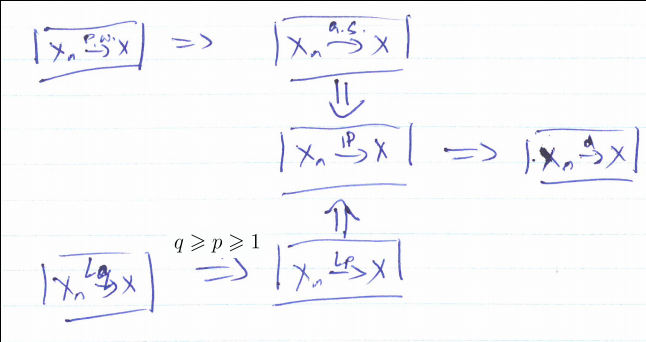
\includegraphics[width=2.5in]{img.png}

\end{multicols*}
\end{document}
